\documentclass[11pt]{article}
\usepackage[margin=1in]{geometry}
\usepackage[T1]{fontenc}
\usepackage{lmodern}
\usepackage{booktabs}
\usepackage{graphicx}
\usepackage{xurl}
\usepackage[hidelinks]{hyperref}
\usepackage[numbers,sort]{natbib}
% Generated by experiments/note_tables.py from results/note/summary.json and step.json.
\newcommand{\TripRows}{
Redmine & Issue list (4 offsets) & 60 & 41 & 41 to 41 & 41 & 0 & 41.0 \\
Redmine & Issue detail & 30 & 20 & 20 to 26 & 20 & 0 & 20.0 \\
Redmine & Project list & 10 & 8 & 8 to 8 & 8 & 0 & 8.0 \\
Redmine & Whole mix & 100 & 41 & 8 to 41 & 41 & 0 & n/a \\
Aimeos & Listing, page 0 (price and name) & 10 & 112 & 112 to 112 & 112 & 1 & n/a \\
Aimeos & Listing, page 1 (price and name) & 10 & 112 & 112 to 112 & 112 & 1 & n/a \\
Aimeos & Listing, page 2 (price and name) & 10 & 39 & 39 to 39 & 39 & 0 & n/a \\
Aimeos & Product detail & 40 & 43 & 43 to 43 & 43 & 1 & 26.0 \\
Aimeos & Whole mix & 100 & 43 & 39 to 112 & 43 & 1 & n/a \\
}
\newcommand{\SlopeRows}{
Redmine & Issue list (4 offsets) & 41.9 & 142.5 & 41 & 52.0 [51.3, 57.3] & 1.27 & 1.27 & 0.987 \\
Redmine & Issue detail & 10.5 & 57.0 & 20 & 23.6 [23.2, 26.9] & 1.18 & 1.18 & 0.997 \\
Redmine & Project list & 6.1 & 25.2 & 8 & 9.8 [9.6, 11.2] & 1.22 & 1.22 & 0.995 \\
Redmine & Whole mix & 39.1 & 138.1 & 41 & 51.3 [50.6, 52.0] & 1.25 & 1.25 & 0.989 \\
Aimeos & Listing, page 0 (price) & 70.3 & 330.1 & 112 & 133.5 [119.6, 147.4] & 1.19 & 1.18 & 0.997 \\
Aimeos & Listing, page 0 (name) & 71.0 & 329.9 & 112 & 133.4 [119.5, 149.0] & 1.19 & 1.18 & 0.997 \\
Aimeos & Listing, page 1 (price) & 71.3 & 330.4 & 112 & 133.2 [119.2, 147.6] & 1.19 & 1.18 & 0.997 \\
Aimeos & Listing, page 1 (name) & 71.6 & 331.0 & 112 & 133.3 [119.2, 148.5] & 1.19 & 1.18 & 0.997 \\
Aimeos & Listing, page 2 (price) & 35.3 & 130.4 & 39 & 49.1 [43.5, 54.7] & 1.26 & 1.26 & 0.996 \\
Aimeos & Listing, page 2 (name) & 35.8 & 130.5 & 39 & 49.1 [43.9, 54.9] & 1.26 & 1.26 & 0.995 \\
Aimeos & Product detail & 36.5 & 144.0 & 43 & 55.5 [49.6, 61.9] & 1.29 & 1.26 & 0.996 \\
Aimeos & Whole mix & 38.8 & 149.2 & 43 & 56.9 [48.0, 62.6] & 1.32 & 1.29 & 0.996 \\
}
\newcommand{\ControlRows}{
Redmine & all 11 settings, 20 runs & 52.0 [51.3, 57.3] & 39.0 & 31.5 & 9.3 & 2.4 & 38.4 \\
Aimeos & all 11 settings, 20 runs & 55.5 [49.6, 61.9] & 85.3 & 69.8 & 18.7 & 3.9 & 84.6 \\
Redmine & control, default & 48.9 [48.2, 49.8] & 37.4 & 31.5 & 7.7 & 2.1 & 37.1 \\
Redmine & slow start after idle off & 49.1 [48.8, 49.8] & 37.5 & 31.5 & 7.7 & 2.1 & 37.1 \\
Redmine & energy preference \texttt{performance} & 43.9 [43.6, 44.2] & 33.7 & 31.5 & 3.7 & 1.6 & 33.6 \\
Redmine & deep idle states blocked & 42.5 [42.2, 42.8] & 32.5 & 31.5 & 2.5 & 1.7 & 32.3 \\
}
\newcommand{\StepRows}{
Redmine & Issue list (4 offsets) & 41 & 0.4 to 0.5 & 11.0 & 1.26 & 1.07 & 1.07 \\
Redmine & Issue detail & 20 & 0.4 to 0.5 & 1.7 & 1.17 & 1.13 & 1.08 \\
Redmine & Project list & 8 & 0.4 to 0.5 & 1.2 & 1.21 & 1.09 & 1.10 \\
Redmine & Whole mix & 41 & 0.4 to 0.5 & 8.7 & 1.24 & 1.07 & 1.07 \\
Aimeos & Listing, page 0 (price) & 112 & 0.5 to 0.75 & 18.1 & 1.19 & 1.05 & 1.09 \\
Aimeos & Listing, page 0 (name) & 112 & 0.5 to 0.75 & 18.5 & 1.19 & 1.06 & 1.08 \\
Aimeos & Listing, page 1 (price) & 112 & 0.5 to 0.75 & 18.3 & 1.19 & 1.05 & 1.09 \\
Aimeos & Listing, page 1 (name) & 112 & 0.5 to 0.75 & 18.8 & 1.19 & 1.06 & 1.08 \\
Aimeos & Listing, page 2 (price) & 39 & 0.5 to 0.75 & 7.3 & 1.26 & 1.06 & 1.14 \\
Aimeos & Listing, page 2 (name) & 39 & 0.5 to 0.75 & 7.9 & 1.26 & 1.06 & 1.13 \\
Aimeos & Product detail & 43 & 0.5 to 0.75 & 9.0 & 1.29 & 1.09 & 1.17 \\
Aimeos & Whole mix & 43 & 0.5 to 0.75 & 8.3 & 1.31 & 1.08 & 1.20 \\
}


\title{Injected Database Round-Trip Time and Page Latency in Redmine and Aimeos}
\author{Akufor Agho Fru}
\date{November 2026}

\begin{document}
\maketitle

\begin{abstract}
This note replicates the queries-times-RTT model of page latency on two unmodified
open-source web applications. On one x86\_64 host (AMD Ryzen AI Max+ 395, Linux 7.2), Linux
\texttt{netem} added the configured round-trip time (RTT) between the application and
PostgreSQL within 0.03~ms from 0.02 to 2~ms. Packet captures gave a fixed number of sequential
database round trips per page, 8 to 112, in Redmine 6.1.4 and Aimeos. With the application,
database, and load client pinned to one CCD, median (p50) page latency rose with injected RTT
in the order of the counts. The least-squares slopes from 0 to 2~ms were 18 to 32\% above the
counts. Most of that excess came from one step, between 0.4 and 0.5~ms RTT in Redmine and
between 0.5 and 0.75~ms in Aimeos, where container CPU time per request also stepped up. Away
from the step, the slopes of single pages were 5 to 17\% above the counts. In single pinned
Redmine control sweeps, holding deep CPU idle states off reduced the issue-list slope to 1.04
times its count. This replicates the queries-times-RTT model and shows that the host power
policy can add to it.
\end{abstract}

\section{Introduction}

Database-backed web pages often run tens of small queries in sequence. When the application
and the database share a process, as with SQLite, this pattern is cheap
\citep{sqlite2026smallqueries}. When they talk over a network, each sequential query adds one
round trip. Platform guidance follows from this: Neon recommends that the application and
database run in the same region \citep{neon2026latency}, and Cloudflare Smart Placement moves
a Worker near its backend because ``the latency from multiple round trips \ldots\ adds up''
\citep{cloudflare2026placement}.

The model itself is not in question. Sloth and Pyxis reduce round trips because each one
costs latency \citep{cheung2014sloth,cheung2012pyxis}, and Sloth measured real ORM
applications at three application-to-database delays. Studies of object-relational mapping
anti-patterns measure the cost of redundant queries \citep{chen2014orm,chen2016redundant,
yang2018hownot}, and link gradients estimate how response time changes with link latency
\citep{chen2011linkgradients}. CPU sleep states and frequency scaling are known to add latency
to short requests \citep{kanev2014tradeoffs,li2014tales,chou2019udpm,hajyahya2022agilewatts,
antoniou2022agilepkgc}. This note adds a public replication in the sub-millisecond range that
a same-zone or same-rack deployment sees, on unmodified applications, where the predicted
slope comes from an independent packet count rather than from the latency curve itself.

The note does not propose a model or a mechanism, and it does not rank frameworks. It answers
three questions:

\begin{enumerate}
  \item[RQ1] Does \texttt{netem} on this host produce the configured RTT at sub-millisecond
    settings?
  \item[RQ2] How many sequential database round trips does each measured page make?
  \item[RQ3] How does the slope of p50 page latency against RTT compare with the round-trip
    count from RQ2, over the whole range and on each side of any step in the curve?
\end{enumerate}

The contributions are:
\begin{enumerate}
  \item A fidelity check of \texttt{netem} from 0.02 to 2~ms, with two probes, two qdisc
    placements, and two kernel controls.
  \item Packet-level round-trip counts for each measured page of Redmine and Aimeos.
  \item Run-level p50 latency over an RTT grid from 0 to 2~ms, with slope fits and bootstrap
    confidence intervals, compared page by page with the counts, and the location of a step
    in the latency curve and in container CPU time per request.
\end{enumerate}

The answers are short. RQ1: yes on this host, with an excess of at most 0.03~ms. RQ2: 8 to
112 round trips per page, fixed for each page. RQ3: the slopes rise in the order of the
counts. Over 0 to 2~ms they are 18 to 32\% above the counts with the containers pinned. The
curve has one step, between 0.4 and 0.5~ms in Redmine and between 0.5 and 0.75~ms in Aimeos,
and container CPU time per request steps at the same place. On each side of the step, the
slopes of single pages are 5 to 17\% above the counts. Section~\ref{sec:limits} lists what
one host and one injection method cannot show.

\section{Prior work}

\paragraph{Round trips as a cost.} Sloth batches queries lazily so that a page needs fewer
round trips \citep{cheung2014sloth}. It reports round trips per page for two real Hibernate
applications, itracker and OpenMRS (for example 59 to 124 per itracker page in its
Section~6.1). Its Section~6.4 varies the delay between the application and database servers
over 0.5, 1, and 10~ms. The round-trip counts stay the same, and the speedup from batching
grows with the delay. Sloth reports speedup ratios, not a per-page slope of latency against
RTT. Pyxis partitions application code between the application server and the database to
reduce control transfers \citep{cheung2012pyxis}. This note fits each page's latency slope on a
finer grid from 0 to 2~ms and compares it with the page's packet-traced count.

\paragraph{ORM anti-patterns.} Chen et al.\ detect ORM anti-patterns such as one-by-one
processing, and measure the response-time gain from fixing them
\citep{chen2014orm,chen2016redundant}. Yang et al.\ study performance bugs in Rails
applications and find that many come from how pages access data \citep{yang2018hownot}.
These studies count or remove queries. They do not vary network RTT.

\paragraph{Latency sensitivity.} Link gradients estimate the derivative of response time
with respect to link latency on running multitier systems with delay injection
\citep{chen2011linkgradients}. That derivative is the slope in RQ3. The present note measures
it at sub-millisecond RTT and compares it with a direct count.

\paragraph{Sub-millisecond injection.} Popescu, Zilberman, and Moore injected latency from
2~$\mu$s to 1~ms with a hardware appliance, because hardware gives ``higher resolution and
better control over latency than software-implemented traffic control such as NetEm might
afford'' \citep{popescu2017latency}. For Ridge Regression on Spark they also added latency with NetEm at
the workers and saw no noticeable effect below 500~$\mu$s RTT. Earlier studies measured the
accuracy of NetEm and other link emulators on older kernels and timers
\citep{nussbaum2009emulators,lubke2014emulators}. RQ1 measures what \texttt{netem} delivers
on the host used here, from 0.02~ms up.

\paragraph{CPU power management and request latency.} Kanev et al.\ show that sleep-state and
frequency choices trade power against request latency in warehouse-scale services
\citep{kanev2014tradeoffs}. Li et al.\ list CPU power saving among the hardware sources of
excess request latency \citep{li2014tales}. $\mu$DPM shows that sleep states and frequency
scaling hurt microsecond-scale service times \citep{chou2019udpm}, and AgileWatts and
AgilePkgC measure deep idle-state wake latency near 100~$\mu$s and its cost for short-wait
services, MySQL among them \citep{hajyahya2022agilewatts,antoniou2022agilepkgc}. These studies
cover the mechanism that the host-setting controls in this note touch. They do not measure
pages that wait on many sequential database round trips.

\paragraph{Practice.} The Neon and Cloudflare documents above give placement advice from the
same model \citep{neon2026latency,cloudflare2026placement}. The SQLite page makes the
complementary point that many small queries are cheap without a network
\citep{sqlite2026smallqueries}.

\section{Method}

\paragraph{Host and applications.} All runs in this note used one x86\_64 host (AMD Ryzen AI
Max+ 395, 16 cores and 32 hardware threads in two CCDs, Linux 7.2.13, Docker 29.8.2,
Compose 5.6.1). The CPU frequency driver was \texttt{amd-pstate-epp} with the
\texttt{powersave} governor, energy preference \texttt{balance\_performance}, and a 2.0 to
5.19~GHz range. In the sweeps of Table~\ref{tab:slopes} and the controls of
Table~\ref{tab:controls}, Docker pinned every container to CCD1: the application to CPUs 8 to 11
and 24 to 27, the database to 12 to 14 and 28 to 30, and the load client to 15 and 31. Other
processes on the host were not pinned and could also run on CCD1. Each run records the busy
time of the pinned CPUs that the two measured containers did not use. Redmine 6.1.4 (Rails, Puma with one
worker process) and Aimeos at commit \texttt{9197200} (Laravel, PHP 8.4 built-in server with
eight workers) each ran against PostgreSQL 18 in its own container. The PostgreSQL, Redmine,
Alpine, and Redmine-side Node.js images are pinned by digest. Two Aimeos images are not: its
application image builds from the \texttt{php:8.4-cli-bookworm} tag, and its probe container
uses the \texttt{node:22-bookworm-slim} tag. The run metadata records the image ID of every
container, and the Aimeos probe ran the same image ID as the pinned Node.js image. The Aimeos
dependencies come from its \texttt{composer.lock}.

\paragraph{Workloads.} Redmine was seeded with 12 projects and 360 issues. Its request mix is
60\% issue lists (four page offsets), 30\% issue details with journals, and 10\% project
lists, through the REST API. Aimeos used its demo catalog. Its mix is 60\% product listings
(two sort orders and three pages) and 40\% product detail pages. A single client in the
application's network namespace sends one request at a time over loopback, so only the
application-to-database link is delayed. These are synthetic request mixes against the real
applications, not production traffic.

\paragraph{RTT injection.} \texttt{netem} adds half of the target RTT on egress in the
application namespace and half in the database namespace. Setting ``none'' removes the qdisc.
Setting 0 installs \texttt{netem} with zero delay. For the fidelity check, the same delays were
also applied on the host-side ends of the two veth pairs (``hostveth''). There, the socket no
longer owns the delayed packets, so TCP small-queue and autocorking effects cannot apply.

\paragraph{RTT measurement (RQ1).} A Node.js client in the application namespace sent
64-byte messages to a TCP echo server in the database namespace and timed each reply. It sent
messages back to back (gap 0) or 1~ms apart, 1{,}000 samples per block, and three blocks per
setting in random order. A second probe timed 500 uncached \texttt{SELECT 1} calls through
the Rails database adapter, two blocks per setting. Two control arms repeated the TCP probe
with TCP autocorking off in both namespaces, and with \texttt{/dev/cpu\_dma\_latency} held at
0, which stopped all entries into the deepest idle state (11{,}653 per second without the
hold and 0 with it).

\paragraph{Round-trip count (RQ2).} At 0, 1, and 2~ms RTT, \texttt{tcpdump} captured the
database port during 100 requests of the measured mix. The client recorded the start and end time of
each request, and each packet was assigned to the request whose time window contained it. A
round trip is a TCP handshake, or a flight of client data that the server answered with
data. A stall is a pause of at least half the RTT inside one side's flight, during which the
other side sent a pure ACK. Such a pause costs an RTT that the flight count misses. At 0~ms the
stall threshold is 0.5~ms, as a control for slow server work. Separately, \texttt{pg\_stat\_statements} counted executed statements per request for
30 requests of each route.

\paragraph{Latency sweep (RQ3).} Twelve conditions (none, and 0, 0.05, 0.1, 0.2, 0.3, 0.4,
0.5, 0.75, 1, 1.5, and 2~ms) each ran 20 times in a seeded random order that interleaves the
conditions. Each run sent 20
discarded warmup requests and then 200 measured requests. Before the first run, one full run
at 0~ms warmed the caches. It is stored, labeled, and excluded from analysis. The unit of
analysis is the run: I take the p50 of each run, overall and for each route or request path
that occurs at least five times per run. For each \texttt{netem} condition I take the median of the run p50 values. The slope is an
ordinary least-squares fit of these 11 medians on configured RTT. The 95\% intervals come from
10{,}000 bootstrap resamples of runs within each condition, with the medians and the fit
recomputed each time. As a stability check, I drop each run in turn and record the largest
change of its condition's median.

\paragraph{CPU accounting.} Before and after each run, the driver reads the cgroup CPU time
of the application and database containers. Before the first run and after the last, it also
measures their CPU time for 60~s with no requests (the idle rate).

\paragraph{Foreign load and the step.} Each run also records the busy time of the pinned CPUs.
That time minus the CPU time of the two measured containers, per second of wall time, is the
load of other processes. Runs where it exceeds 2 hardware threads are loaded runs. To locate a
step, I take the condition medians of run p50 over the runs without foreign load, and find the
adjacent pair of settings whose rise exceeds the median rise per ms of RTT by the most. I then
fit the settings below the lower edge of that pair and the settings from its upper edge to
2~ms separately (\texttt{experiments/step\_note.py}).

\section{Results}

\subsection{RQ1: \texttt{netem} produces the configured RTT on this host}

On the x86\_64 host, the added p50 RTT of back-to-back TCP echoes stayed within 0.029~ms of the
setting at every point from 0.02 to 2~ms (Table~\ref{tab:fidelity}, Figure~\ref{fig:fidelity}).
For Rails \texttt{SELECT 1} the excess was at most 0.034~ms up to 1~ms and 0.059~ms at 2~ms. Back-to-back TCP echoes
gained 0.0524~ms at a 0.05~ms setting and 1.0165~ms at 1~ms. The Rails \texttt{SELECT 1}
probe, which adds driver and adapter work, gained 0.0627 and 1.0336~ms. \texttt{netem} with
0~ms delay was indistinguishable from no qdisc (0.0136 against 0.0134~ms p50). The p95 stayed
within 0.10~ms of the p50 for both probes at 0.5~ms and below.

This is a direct measurement of \texttt{netem} below 500~$\mu$s, where the hardware study
above chose not to rely on software injection \citep{popescu2017latency}. On this host and
kernel, \texttt{netem} resolved settings of 20~$\mu$s and up. None of the three suspected
artifacts changed this. Moving the qdisc to the host-side veth,
turning off TCP autocorking, and blocking deep idle states each moved the added p50 RTT by at
most 0.025~ms at any setting. A 1~ms pause between echoes, which lets cores go idle, also left
the excess at 0.035~ms or less up to 1~ms. On this host, the sub-millisecond points need no
fence.

\begin{table}[t]
\centering
\caption{Measured p50 and p95 RTT (ms) at each \texttt{netem} setting on the x86\_64 host. TCP
echo: 3{,}000 back-to-back samples per setting. Rails \texttt{SELECT 1}: 1{,}000 samples per
setting. ``Added'' is p50 minus the p50 with no qdisc. Source: run
\texttt{2026-11-18-netem-fidelity}.}
\label{tab:fidelity}
\begin{tabular}{lrrrrrr}
\toprule
& \multicolumn{3}{c}{TCP echo} & \multicolumn{3}{c}{Rails \texttt{SELECT 1}} \\
\cmidrule(lr){2-4}\cmidrule(lr){5-7}
Setting & p50 & p95 & Added & p50 & p95 & Added \\
\midrule
none & 0.0134 & 0.0219 & 0 & 0.0262 & 0.0382 & 0 \\
0    & 0.0136 & 0.0239 & 0.0002 & 0.0266 & 0.0513 & 0.0004 \\
0.02 & 0.0361 & 0.0571 & 0.0227 & 0.0548 & 0.0792 & 0.0286 \\
0.05 & 0.0658 & 0.0951 & 0.0524 & 0.0889 & 0.1457 & 0.0627 \\
0.1  & 0.1298 & 0.1528 & 0.1164 & 0.1505 & 0.2068 & 0.1243 \\
0.2  & 0.2185 & 0.2642 & 0.2051 & 0.2407 & 0.3053 & 0.2145 \\
0.3  & 0.3226 & 0.3693 & 0.3092 & 0.3405 & 0.4231 & 0.3143 \\
0.5  & 0.5199 & 0.5675 & 0.5065 & 0.5539 & 0.6428 & 0.5277 \\
1    & 1.0299 & 1.0983 & 1.0165 & 1.0598 & 1.1732 & 1.0336 \\
2    & 2.0420 & 2.1279 & 2.0286 & 2.0852 & 2.2485 & 2.0590 \\
\bottomrule
\end{tabular}
\end{table}

\begin{figure}[t]
\centering
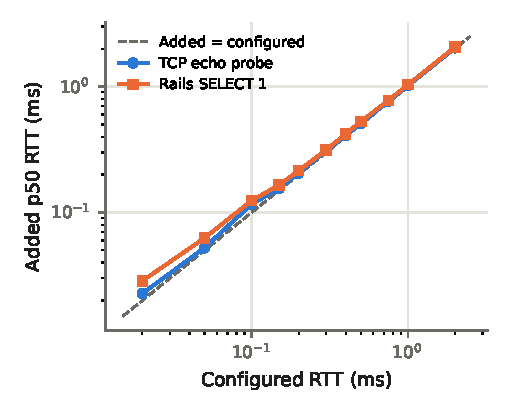
\includegraphics[width=0.48\linewidth]{figures/netem_fidelity.pdf}
\caption{Added p50 RTT against the \texttt{netem} setting on the x86\_64 host, log scales. The
dashed line is equality. Both probes track it from 0.02 to 2~ms.}
\label{fig:fidelity}
\end{figure}

\paragraph{The earlier ARM64 host did not deliver small settings faithfully.} An earlier
Redmine sweep on an ARM64 host (Cortex-X925, Linux 7.0) showed a 9.3~ms step in p50 between 0
and 0.05~ms. The same fidelity phase on that host (run
\texttt{2026-11-18-netem-fidelity-arm64-host}) shows that its injected RTT was not the
configured RTT at small settings. With the default idle states, back-to-back echoes at 0.02 to
0.15~ms settings took 0.251 to 0.307~ms at p50 and 0.75 to 0.93~ms at p95. With
\texttt{/dev/cpu\_dma\_latency} held at 0, the same settings gave 0.076~ms at 0.05 and
0.152~ms at 0.1. That run's autocorking arm did not start because a container failed to
initialize, but the default, \texttt{SELECT 1}, and idle-state arms completed. The earlier
Redmine sweep was not repeated with deep idle states blocked, so this note does not attribute
its step to a cause. It excludes all ARM64 application results and uses only the x86\_64
runs.

\subsection{RQ2: each page makes a fixed number of sequential round trips}

The packet traces give each page a fixed count (Table~\ref{tab:trips}). In Redmine, each
round trip carries one statement: 41 for every issue-list page, 20 for an issue detail, and 8
for the project list. \texttt{pg\_stat\_statements} agrees (41.0, 20.0, and 8.0 statements per
request). Redmine reuses pooled connections, so its requests had no TCP handshakes. Aimeos
opens three new database connections per request, and it makes more round trips than
statements. A product detail page took 43 round trips for 26 statements, because connection
setup and authentication add round trips that are not statements. Listing pages 0 and 1 took
112 round trips, and page 2 took 39. The counts did not change with RTT: the medians at 0, 1,
and 2~ms were equal for every page.

Stalls inside a flight, where one side waits for a pure ACK, were rare. Redmine pages had none.
Aimeos listing pages 0 and 1 and the product detail page had one such stall at 1 and 2~ms RTT,
and listing page 2 had none. A stall costs one RTT, so Table~\ref{tab:slopes} also gives each
ratio with the stalls counted as round trips.

\begin{table}[t]
\centering
\caption{Sequential database round trips per request from packet capture. Requests: traced
requests per page at each RTT. Range: minimum to maximum at 0~ms. Stalls: median pauses that
waited for a pure ACK at 2~ms. Statements: \texttt{pg\_stat\_statements} calls per request for
30 requests of the route. Source: runs \texttt{2026-11-18-redmine-stall-trace} and
\texttt{2026-11-18-aimeos-stall-trace}. The earlier traces without stall counts gave the same
medians.}
\label{tab:trips}
\footnotesize
\setlength{\tabcolsep}{4pt}
\begin{tabular}{llrrrrrr}
\toprule
App & Page & Requests & RT at 0 & Range & RT at 2 & Stalls & Statements \\
\midrule
\TripRows
\bottomrule
\end{tabular}
\end{table}


\subsection{RQ3: slopes follow the counts, with a step}

Every 0 to 2~ms slope exceeds its page's round-trip count, and no count falls inside its
slope's 95\% interval (Table~\ref{tab:slopes}, Figure~\ref{fig:slopes}). With the containers
pinned to CCD1 and 20 runs per condition, the slope is 1.18 to 1.27 times the count for single
Redmine pages and 1.25 times for the Redmine mix, which takes its median from the
41-round-trip issue list. In Aimeos it is 1.19 for listing pages 0 and 1, 1.26 for page 2,
1.29 for the product detail route, and 1.32 for the mix. With each Aimeos stall counted as a
round trip, the Aimeos ratios are 1.17 to 1.28 for pages and paths and 1.29 for the mix. The
slopes keep the order of the counts: 9.8, 23.6, and 52.0~ms per ms for 8, 20, and 41 round
trips in Redmine, and 49.1, 55.5, and about 133.4~ms per ms for 39, 43, and 112 in Aimeos.
Each count holds for both sort orders of a listing page, and the two sort orders give slopes
within 0.3~ms per ms of each other.

\paragraph{The curve has a step.} The 0 to 2~ms fit puts one line through a curve that is not
one line. In the runs without foreign load, the median p50 of the Redmine issue list rose from
60.2~ms at 0.4~ms RTT to 75.7~ms at 0.5~ms, where 41 round trips predict 4.1~ms. The Aimeos
product detail rose from 59.4~ms at 0.5~ms to 80.6~ms at 0.75~ms, where 43 round trips predict
10.8~ms. Every page has its largest rise above trend between the same two settings as its
mix (Table~\ref{tab:step}). Below and above the step, the slopes are close to the counts. The
Redmine issue list gives 1.07 times its count below the step and 1.07 above it. The Aimeos
product detail gives 1.09 below and 1.17 above. Over all single pages, the off-step slopes are
1.05 to 1.17 times the counts. Most of the 18 to 32\% excess of the 0 to 2~ms fit is
therefore the step, not a fixed extra cost per ms of RTT. The $r^2$ of 0.987 to 0.997 of the
0 to 2~ms fits does not show that the curve is a line.


\paragraph{Foreign load.} The sweeps ran on a shared host. Other processes used more than 2 of
the 16 pinned hardware threads in 49 of 240 Redmine runs and 67 of 240 Aimeos runs, and up to
15.6 threads. In 21 Redmine runs and 50 Aimeos runs, the run p50 was more than 1.5 times its
condition median, and every one of these runs was a loaded run. The median-based slopes change
little without the loaded runs: the issue-list slope goes from 52.0 to 51.7, the
product-detail slope stays at 55.5, and the page-0 listing slope goes from 133.5 to 133.4.
Dropping any single run moved a condition median by at most 0.50 of that condition's 95\%
half-width. Table~\ref{tab:step} and the CPU accounting below use the runs without foreign
load.

An earlier unpinned sweep, with 10 runs per condition and the containers free to use all
32 threads, gave other 0 to 2~ms ratios: 1.26 to 1.39 for Redmine pages and 1.12 for the
Aimeos listing and detail routes. Placement on the CPU changes the size of the excess in both
directions.

\begin{table}[t]
\centering
\caption{Run-level p50 page latency and the fitted RTT slope, containers pinned to CCD1, all
runs. p50 values are medians over 20 runs of 200 requests. The slope is ms of p50 per ms of
RTT, fitted through the medians at the 11 \texttt{netem} settings from 0 to 2~ms, with a
bootstrap 95\% interval. RT: traced round trips (Table~\ref{tab:trips}). Ratio: slope divided
by RT. +Stalls: slope divided by RT plus the median stalls at 2~ms. $r^2$ of the straight-line
fit, which does not detect the step of Table~\ref{tab:step}. Sources: runs
\texttt{2026-11-18-redmine-rtt-sweep-pinned} and \texttt{2026-11-18-aimeos-rtt-sweep-pinned}.}
\label{tab:slopes}
\footnotesize
\setlength{\tabcolsep}{4pt}
\begin{tabular}{llrrrlrrr}
\toprule
App & Page & p50 at 0 & p50 at 2 & RT & Slope [95\% CI] & Ratio & +Stalls & $r^2$ \\
\midrule
\SlopeRows
\bottomrule
\end{tabular}
\end{table}

\begin{figure}[t]
\centering
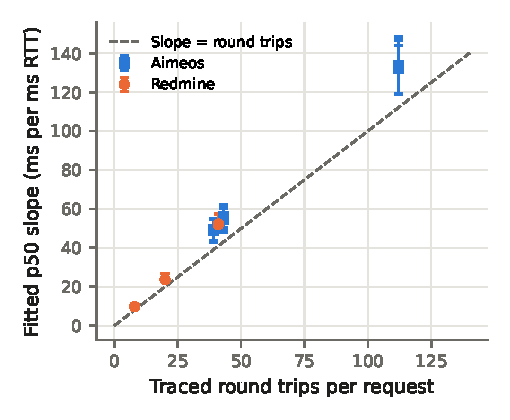
\includegraphics[width=0.48\linewidth]{figures/slope_vs_round_trips.pdf}
\caption{Fitted 0 to 2~ms p50 slope against traced round trips per request, with 95\%
intervals, containers pinned to CCD1. Points are request paths and routes. The dashed line is
slope equal to round trips. All points lie above it.}
\label{fig:slopes}
\end{figure}

\begin{table}[t]
\centering
\caption{Slopes on each side of the step, containers pinned to CCD1, runs without foreign
load (177 Redmine and 158 Aimeos \texttt{netem} runs). Step: the adjacent pair of settings
with the largest rise of the mix median above the median rise per ms. Rise: that rise for the
page, in ms. Ratio columns divide a slope by the traced round trips (RT). 0 to 2: all 11
settings. Below: settings under the lower edge of the step. Above: settings from the upper
edge to 2~ms. Source: \texttt{results/note/step.json} from
\texttt{experiments/step\_note.py}.}
\label{tab:step}
\footnotesize
\setlength{\tabcolsep}{4pt}
\begin{tabular}{llrlrrrr}
\toprule
App & Page & RT & Step (ms) & Rise & 0 to 2 & Below & Above \\
\midrule
\StepRows
\bottomrule
\end{tabular}
\end{table}

\paragraph{CPU time steps at the same place.} The excess is not in the network path. The
\texttt{netem} excess over the setting is at most 0.029~ms at 2~ms, under 2\% of the slope
(RQ1), and the packet traces show at most one ACK-clocked stall per page (RQ2). Measured
container CPU time per request steps where latency steps. In the pinned Redmine sweep, the
median over runs of the application plus database CPU time per request was 29.7~ms at 0~ms,
32.2~ms at 0.4~ms, 40.1~ms at 0.5~ms, and 45.8~ms at 2~ms. In Aimeos it was 59.0~ms at 0~ms,
60.0~ms at 0.5~ms, 74.1~ms at 0.75~ms, and 90.6~ms at 2~ms. The runs without foreign load
place the CPU step between the same settings.

The CPU time also gives an approximate account of the mean-latency slope. With no requests,
the two containers used 0.061~ms of CPU per ms of wall time in Redmine and 0.046 in Aimeos,
measured for 60~s before and after each sweep. A slower request collects more of this idle
CPU, so it is removed. In the Redmine runs without foreign load, mean round trips (31.5) plus
the CPU slope (9.3) minus idle CPU (2.4) give 38.4~ms per ms, against a slope of mean latency
of 39.0. In Aimeos the same sum is 69.8 plus 18.7 minus 3.9, or 84.6, against 85.3
(Table~\ref{tab:controls}). The two agree within 2\%. The CPU time is measured. That it sits
on the request path is inferred: one client sends one request at a time, but cgroup time also
counts work beside the request.

\begin{table}[t]
\centering
\caption{CPU accounting, containers pinned to CCD1. The first two rows are the sweeps of
Table~\ref{tab:slopes}. Their Mean, CPU, Idle, and Sum columns use the runs without foreign
load (Table~\ref{tab:step}). Each control is one sweep of 10 runs of 200 requests at 0, 0.5,
1, and 2~ms, and the four controls ran once each, one after another. Slope: p50 slope of the
Redmine issue list or the Aimeos product detail over all runs, with 95\% interval. Mean: slope
of run-mean latency over the mix. RT: mean round trips per request. CPU: slope of container
CPU time per request. Idle: idle CPU collected per ms of RTT. Sum: RT plus CPU minus Idle. All
slopes are in ms per ms of RTT.}
\label{tab:controls}
\footnotesize
\setlength{\tabcolsep}{4pt}
\begin{tabular}{lllrrrrr}
\toprule
App & Run & Slope [95\% CI] & Mean & RT & CPU & Idle & Sum \\
\midrule
\ControlRows
\bottomrule
\end{tabular}
\end{table}

\paragraph{Host-setting controls.} Each pinned Redmine control is one sweep at 4 RTT settings
(0, 0.5, 1, and 2~ms) with 10 runs per setting, and the four sweeps ran once each, one after
another. Four settings cannot locate the step. With the default settings, the issue-list slope
was 48.9 [48.2, 49.8] and the CPU slope 7.7. With the CPU energy-performance preference held
at \texttt{performance}, they were 43.9 [43.6, 44.2] and 3.7. With deep idle states held off
through \texttt{/dev/cpu\_dma\_latency}, they were 42.5 [42.2, 42.8] and 2.5, so the
issue-list slope was 1.04 times its 41 round trips. Turning off TCP slow start after idle
changed nothing (49.1 and 7.7). Other processes used at most 0.82 of the pinned threads in
every run of the last three controls, and more than 1 thread in 4 of the 40 default-control
runs (up to 6.3). Earlier unpinned controls with 5 runs per setting showed no effect of the
same settings: all their issue-list slopes were 55.4 to 57.4.

\section{Discussion}

On these pages, the slopes of p50 latency against injected RTT follow the order of the traced
round-trip counts, and away from the step they are 5 to 17\% above the counts. On this host and with this pinning, the curve also has one step, between
0.4 and 0.5~ms RTT in Redmine and between 0.5 and 0.75~ms in Aimeos, and container CPU time
per request steps at the same place. In the single pinned Redmine control sweeps, holding deep
idle states off brought the issue-list slope to 1.04 times its count. The unpinned controls
showed no such effect, so these runs tie the step to the power policy only for the pinned
configuration on this host. The mechanism itself, that CPU sleep states and frequency scaling
add latency to requests that wait on short gaps, is established
\citep{kanev2014tradeoffs,li2014tales,chou2019udpm,hajyahya2022agilewatts}. This note shows
that the same effect can appear in the RTT response of a database-bound page.

The earlier ARM64 host is a second reason to check the injected RTT. There, \texttt{netem}
settings from 0.02 to 0.15~ms produced p50 echo times of 0.25 to 0.31~ms unless deep idle
states were blocked. An RTT injection study should check the injected RTT with an independent
probe on the same host, should report the host's CPU placement and its idle and frequency
settings, and should fit the curve on a grid fine enough to show a step.

\section{Limits}
\label{sec:limits}

\begin{itemize}
  \item One host. Absolute latencies, the size of the excess, and the place of the step depend
    on this CPU, its power policy, and the placement of the containers.
  \item The host was shared. Other processes loaded the pinned CPUs in 49 of 240 Redmine runs
    and 67 of 240 Aimeos runs.
  \item Each pinned control setting ran once, at 4 RTT settings.
  \item Only \texttt{netem} delay, with no jitter, loss, reordering, or bandwidth limit, and no
    cloud network. The note measures sensitivity to RTT, not the RTT of any provider.
  \item One client at a time.
  \item Synthetic request mixes on two applications with small seeded data sets. The round-trip
    counts are properties of these pages, not of Rails or Laravel in general.
  \item The fidelity probe and the packet traces ran without CPU pinning.
\end{itemize}

\section{Conclusion}

On one x86\_64 host, \texttt{netem} added the configured RTT within 0.03~ms from 0.02 to 2~ms,
and packet captures gave fixed sequential database round-trip counts of 8 to 112 per page in
Redmine 6.1.4 and Aimeos. With the containers pinned to one CCD, p50 page latency rose with
injected RTT in the order of the counts, and the 0 to 2~ms slopes were 18 to 32\% above the
counts. Most of that excess came from a step between 0.4 and 0.75~ms RTT, where container CPU
time per request also stepped up. Away from the step, single-page slopes were 5 to 17\% above
the counts. In single pinned Redmine control sweeps, holding deep CPU idle states off reduced
the issue-list slope to 1.04 times its count. This replicates the queries-times-RTT model and
shows that the host power policy can add to it.

\section{Reproduction}

The project \texttt{README.md} lists the commands. The run directories hold raw data, the
seeded condition order, the environment, and SHA-256 hashes of the scripts. The project has
no version control, so these hashes identify the code version.

\bibliographystyle{plainnat}
\bibliography{references}
\end{document}
